% Chapter 4

\chapter{Experiments}
\label{Chapter4}

In order to assess the quality of the methodology described in Section \ref{sec:method},
we tested it on several commonly adopted benchmarks and against a baseline method
that is detailed in the following sections.

\section{Datasets}
\label{subsec:datasets}

The experiments were conducted on five different datasets, namely:
AIDS \cite{Weislow19041989}, CAS\footnote{http://cheminformatics.org/datasets/bursi/},
CPDB \cite{journals/jcisd/HelmaCKR04}, GDD \cite{dobson2003}, and NCI1 \cite{journals/kais/WaleWK08}.
All these datasets contain chemical and molecular particles encoded in graph form,
all the nodes are labelled and none have self loops, that is an edge going in and 
out the same node.
The AIDS Antiviral Screen dataset contains chemical compounds, labelled according to
their antiviral activity; CAS and CPDB are datasets of mutagenic
compounds; NCI1 consists of chemical compounds screened for activity against 
non-small lung cancer cells; GDD is composed of X-ray crystal structures of
proteins represented as graphs.
    \begin{table}[ht]
        \centering
        \begin{tabular}{|r|r|r|r|r|}
            \hline
            Dataset & n. of graphs & sample split & avg nodes & avg edges \\ \hline
            AIDS    & 1503         & 28.07        & 58.90     & 61.40     \\ \hline      
            CAS     & \textbf{4337} & 55.36        & 29.90     & 30.90     \\ \hline      
            CPDB    &  684         & 49.85        & 14.10     & 14.60     \\ \hline      
            GDD     & 1503         & 58.65        & 284.31    & \textbf{2862.63}   \\ \hline      
            NCI1    & 1503         & 50.04        & 29.87     & 32.30     \\ \hline      
        \end{tabular}
        \caption{Statistics about the datasets employed in the experiments: number
        of graphs, labels percentage among samples, average number of nodes, average
        number of edges.}
        \label{table:datasets}
    \end{table}

Some statistics about these datasets are reported in table~\ref{table:datasets},
from this data it is clear that the CAS and NCI1 datasets are the bigger ones
while the GDD holds the most complex graphs.
Furthermore the AIDS dataset turns out to be quite unbalanced in terms of labels
distribution \cite{rtesselli}.  

%----------------------------------------------------------------------------------------

\section{Experiments description}
\label{sec:description}

All the experiments exposed in this section consist in a nested k-fold
cross-validation routine.
The $k$ parameter of the cross-validation is fixed at 10 since this value
already provides good statistical significance while helping containing the bias
skewing during the training phase.
Moreover, the whole routine is run ten times with ten different splits of the
data in order to mitigate the high variance derived during the testing phase due to the
chosen value of $k$.

\subsection{Baselines}
\label{subsec:baselines}
% what
The baseline method to which we compare our methodology is a regular hyper-parameter selection
performed through a grid search (Section \ref{subsubsec:grid}).
The employed classifier is the Support Vector Machine (Section \ref{subsubsec:svm}).
The kernels tested with this method are:
\begin{itemize}
    \item $ODDK_{ST}$ (Section \ref{subsubsec:odd}), $TCK_{ST}$ (Section \ref{subsec:context}), and the kernel resulting
        from their sum (Section \ref{subsubsec:odd});
    \item $ODDK_{ST+}$ (Section \ref{subsubsec:odd}), $TCK_{ST+}$ (Section \ref{subsec:context}) and their sum;
    \item $WL$ (Section \ref{subsubsec:fs}), $WLC$ (Section \ref{subsec:context}) and their sum.
\end{itemize}

% how &  why
This method performs a standard hyper-parameter selection using an exhaustive search
on a finite subset of the parameter space deriving from the composition of the
kernel function and kernel machine respective spaces.
We compare the method performances with a single kernel function and with the
kernel resulting from the sum of two kernel functions that is a combination of the two.
This combination is reproposed in the experiments employing the new method altough
the resulting feature space is a composition rather than a union.

Each kernel function is used to train a SVM classifier whose $C$ parameter
was validated on the set $\{10^{-4},10^{-3},\dots,10^3\}$.
The kernel functions parameters where validated on the following sets:
\begin{itemize}
    \item for the kernels derived from the $ODD$ framework:
    \begin{itemize}
        \item $h=\{1,\dots,10\}$ and 
        \item $\lambda=\{0.1, 0.5, 0.8, 0.9, 1.0, 1.1, 1.2, 1.3, 1.4, 1.5, 1.8\}$,
    \end{itemize}
    \item for the kernels derived from the $WL$ framework:
    \begin{itemize}
        \item $h=\{1,\dots,10\}$.
    \end{itemize}
\end{itemize}
The parameter sets both for the kernels and the classifier are taken from \cite{rtesselli}.

Moreover, for the first combination of the list ($ODDK_{ST}$ and $TCK_{ST}$)
we compare our results against those in \cite{gmkl} which are:

\begin{itemize}
    \item the $ODD-MKL$ kernel with EasyMKL as the kernel machine, and
    \item the $ODD_{ST}$ kernel with SVM as the kernel machine.
\end{itemize}

These experiments perform a hyper-parameter selection employing both a single and 
a multiple kernel learning approach using two of the kernel functions selected here.
In particular the experiments concerning the $ODD-MKL$ kernel use a setup similar to
our methodology while employing only the kernels computed from a single tuple of
parameters coming from the grid for each experiment.
The experiments carried on in \cite{gmkl} employ a slightly different parameter grid
than the one used here, namely the $h$ parameter of the $ODD-MKL$ and $ODDK_{ST}$ is
validated on the set $\{1,\dots,8\}$, the parameter $\lambda$ of the $ODDK_{ST}$ is 
validated on the set $\{0.5,0.6,\dots,1.6\}$ and the $C$ parameter of the SVM
is validated on the set $\{10^{-3},10^{-2},\dots,10^4\}$.

\subsection{The proposed method}
\label{subsec:firstg}

These experiments aim to test the basic methodology proposed in Section \ref{sec:method},
in other words they implement the scheme in Figure \ref{fig:comp2}.
The kernels selected for this set of experiments are:
\begin{enumerate}
    \item the $ODDK_{ST}$ (Section \ref{subsubsec:odd}) and $TCK_{ST}$ (Section \ref{subsec:context}) graph kernels,
    \item the $ODDK_{ST+}$ (Section \ref{subsubsec:odd}) and $TCK_{ST+}$ (Section \ref{subsec:context}) graph kernels,
    \item the $WL$ (Section \ref{subsubsec:fs}) fast subtree and $WLC$ (Section \ref{subsec:context}) graph kernels.
\end{enumerate}
The kernel machine employed is EasyMKL (Section \ref{subsec:easymkl}).
These kernels are also tested in combination that is, the kernels resulting from
two different functions are employed together in a single experiment.

The kernels derived from the $ODD$ framework are calculated according to a parameters grid
composed from the sets:
\begin{itemize}
    \item $h=\{1,\dots,10\}$ and 
    \item $\lambda=\{0.1, 0.5, 0.8, 0.9, 1.0, 1.1, 1.2, 1.3, 1.4, 1.5, 1.8\}$,
\end{itemize}
both sets are taken from \cite{rtesselli}.
To calculate the kernels derived from the $WL$ framework a grid corresponding to
the set $h=\{1,\dots,10\}$ is employed, where $h$ is the only hyper-parameter of
the $WL$ kernels, see Section \ref{subsubsec:fs}.

The hyper-parameter selection is done only for the kernel machine and refers
to the parameter grid derived from the set $\Lambda=\{0.0, 0.1,\dots,1.0\}$, $\Lambda$
being the only hyper-paramter of the EasyMKL algorithm.

\subsection{The proposed method with kernel orthogonalization}
\label{subsec:secondg}
%Section \ref{subsec:features}.

% add more motivations behind these experiments.
The experiments to test the improved methodology proposed in Section \ref{subsec:features}
reflect the list of those in Section \ref{subsec:firstg}.
The set of kernel matrices is pre-computed for each of the possible combinations
of a parameter grid thus defined:

\begin{itemize}
    \item for the kernels derived from the $ODD$ framework:
    \begin{itemize}
        \item $h=\{1,\dots,10\}$
        \item the $\lambda$ parameter was fixed to 1 for the reasons explained in \ref{subsec:features}
    \end{itemize}
    \item for the kernels derived from the $WL$ the parameter $h$ was set to 10
        given the nature of the orthogonalization applied to this kernel (see Section \ref{subsec:features}).
\end{itemize}
The parameter sets both for the kernels and the classifier are taken from \cite{rtesselli}.
For all the experiments, the $\Lambda$ parameter of EasyMKL is
validated on the set $\{0.0, 0.1,\dots,1.0\}$ during the cross-validation
routine.

\paragraph{The case of the GDD dataset:}
\label{par:gdd}
confirming the experience reported in \cite{rtesselli}, while working with the GDD
dataset and the $ODD$ kernels we had to limit the $h$ hyper-parameter to the set
$\{1,2,3\}$ because for heights greater than 3 the computational times of the
kernel matrices became prohibitive, due to the high complexity and magnitude
of the data structures contained in this dataset.

%----------------------------------------------------------------------------------------

\section{Results and discussion}
\label{sec:results}

\subsection{Notation}
\label{subsec:notation}
Given the number of experiments presented, they have been grouped according
to the employed method.
The group is indicated as an apex on the kernel names considered from time to time, with the following meaning:
\begin{itemize}
    \item the group labelled $\boldsymbol{hs}$ refers to the experiments where a standard
        \textbf{h}yper-parameter \textbf{s}election is performed, i.e. the baseline experiments (Section \ref{subsec:baselines});
\item the group labelled $\boldsymbol{c}$ refers to the experiment conducted \textbf{c}ombining the 
        kernels with EasyMKL, i.e. the proposed method (Section \ref{subsec:firstg});
\item the group labelled $\boldsymbol{oc}$ refers to the experiments concerning the \textbf{o}rthogonalized
        kernels \textbf{c}ombination with EasyMKL i.e. the improvement over the proposed method (Section \ref{subsec:secondg}).
\end{itemize}

\subsection{Space resources requirements}
Given the large number of kernel matrices involved in the combination exepriments
we would like to detail the space resources requirements that these experiments
have when the basic methodology (\ref{subsec:firstg}) and the improved one (\ref{subsec:secondg})
are applied.
Table \ref{table:mem1} shows the data obtained in the first case while \ref{table:mem2} shows
the data obtained after applying the kernel orthogonalization strategy.
The data shown here only concerns the $ODD_{ST}$ and $TCK_{ST}$ kernels since for the 
other $ODD$-derived kernels the numbers are basically the same.
The $WL$ and $WLC$ kernel both generated the same amount of matrices in both cases
due to the variation in the parameter grids described above.

\begin{table}[ht]
    \centering\footnotesize
    \begin{tabular}{|l|l|r|r|r|r|r|r|}
        \hline
        $\mathrm{(kernels)^{method}}$ & n. of kernels & AIDS & CAS & CPDB & GDD & NCI1 \\
        \hline
        $(ODDK_{ST})^c$ & 110 & 5 GB & 32 GB & 2 GB & 1 GB & 24 GB \\
        \hline
        $(TCK_{ST})^c$ & 110 & 5 GB & 32 GB & 2 GB & 1 GB & 24 GB \\
        \hline
        $(ODDK_{ST}, TCK_{ST})^c$ & 220 & 10 GB & 56 GB & 5 GB & 3 GB & 48 GB \\
        \hline
    \end{tabular}
    \caption{\footnotesize The number of computed kernels matrices and the memory
    occupation in GigaBytes for each dataset during the experiments described in
    Section \ref{subsec:firstg}.}
    \label{table:mem1}
\end{table}
\begin{table}[ht]
    \centering\footnotesize
    \begin{tabular}{|l|l|r|r|r|r|r|r|}
        \hline
        $\mathrm{(kernels)^{method}}$  & n. of kernels & AIDS & CAS & CPDB & GDD & NCI1 \\
        \hline
        $(ODDK_{ST})^{oc}$ & 65 & 3 GB & 19 GB & <2 GB & <1 GB & 17 GB \\
        \hline
        $(TCK_{ST})^{oc}$ & 65 & 3 GB & 19 GB & <2 GB & <1 GB & 17 GB \\
        \hline
        $(ODDK_{ST}, TCK_{ST})^{oc}$ & 130 & 5 GB & 34 GB & 3 GB & <2 GB & 29 GB \\
        \hline
    \end{tabular}
    \caption{\footnotesize The number of computed kernels matrices and the memory
    occupation in GigaBytes for each dataset during the experiments described in 
    Section \ref{subsec:secondg}.}
    \label{table:mem2}
\end{table}

Time resources requirements being a part of the proposed improvements is given
in Section \ref{subsec:time_results}.

\subsection{Analysis of computational times}
\label{subsec:time_results}

The plot in figure~\ref{fig:times} shows the relation between the computation times
for the $ODD_{ST}\text{ and }TCK_{ST}$ kernels combination on the benchmark datasets,
using Algorithm \ref{alg:incremental} detailed in Section \ref{subsec:inc}.
See Section~\ref{subsec:datasets} for further details on the composition of each dataset.
This data has been collected from experiments run on the same machine.
From the plot it is clear that the complexity of computing the kernel in an incremental
fashion does not grow linearly with the number of kernels being computed.

\begin{figure}[ht]
    \centering
    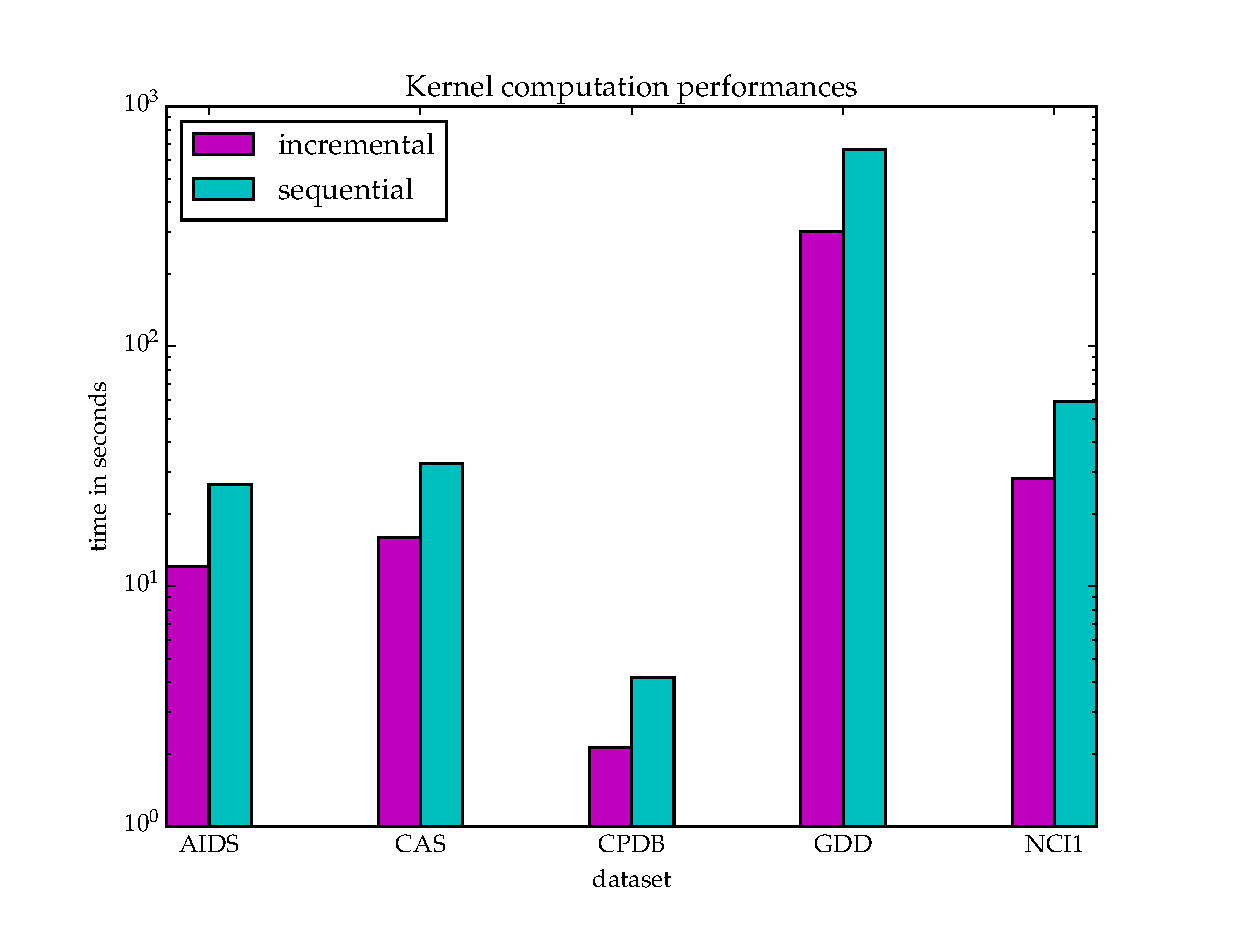
\includegraphics[scale=0.5]{Figures/kernel_times_log}
    \caption{Log time in seconds required to compute the kernels $ODD_{ST}$ and 
    $TCK_{ST}$ incrementally and sequentially on a selection of datasets.}
    \label{fig:times}
\end{figure}

We now present an analysis of the computational time performances of the proposed methodology
with respect to the baseline method. To keep the results comparable we consider only those
experiments employing the same kernels and the same setup, that is:

\begin{itemize}
    \item $(TCK_{ST})^{hs}$, $(TCK_{ST})^c$, and $(TCK_{ST})^{oc}$
    \item $(TCK_{ST+})^{hs}$, $(TCK_{ST+})^c$, and $(TCK_{ST+})^{oc}$
    \item $(WLC)^{hs}$, $(WLC)^c$, and $(WLC)^{oc}$
\end{itemize}

This data has been collected by experiments run on two identical machines.

\begin{figure}[ht]
    \centering
    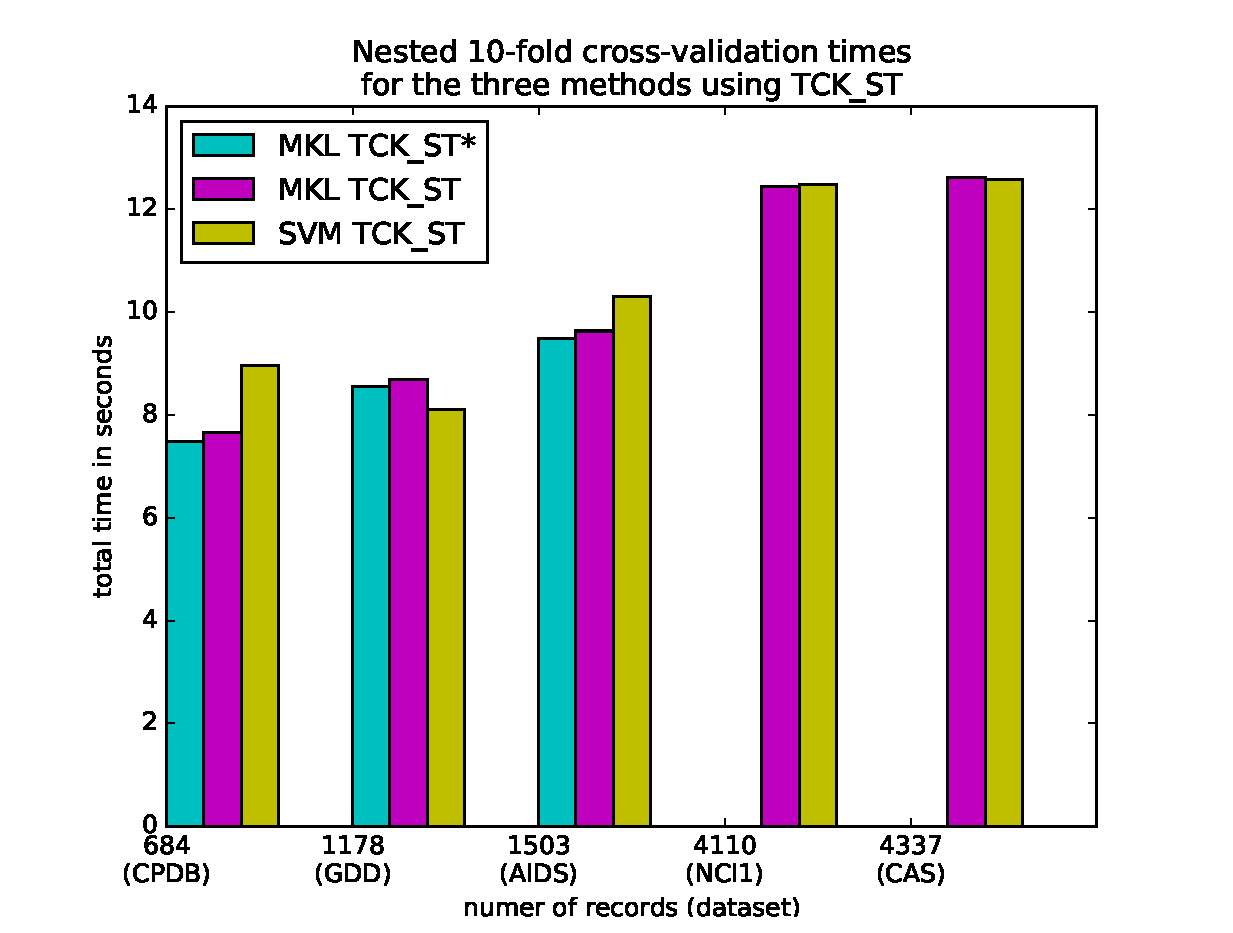
\includegraphics[scale=0.7]{Figures/total_times}
    \caption{
        This plot shows the time required by each method to compute a full nested 10-fold cross-validation on the benchmark datasets.
        The data shown here refers only to the experiments conducted employing the $TCK_{ST}$ kernel.
    }
    \label{fig:datasetstimes}
\end{figure}

As one can see from Figure \ref{fig:datasetstimes}, the proposed methodology is more
efficient in general with respect to the baseline method.
In this case, $(TCK_{ST})^{oc}$ register a 36.4\% average
decrement in the overall time required to perform a full nested 10-fold cross
validation with respect to the standard method, i.e. $(TCK_{ST})^{hs}$.
The only case where the proposed methodology fares worse is with the GDD dataset.
This can be ascribed to the particular case that this dataset represents that is, due to the parameters
set limitation in this case, less kernels are generated w.r.t. the other datasets
and this deeply affects the hyper-parameter selection process while being of no relevance for
EasyMKL, that remains linear in the input size.
From this data we can finally conclude that our methodology is more susceptible
to dataset dimension variation (i.e. the number of samples) while the single-kernel
method is ideed influenced by the same measure but it is even more influenced by
the dimensions of the parameters grid.

The data shown in Figure \ref{fig:datasetstimes2} is in agreement with the data
in figure \ref{fig:datasetstimes}; we register smaller time durations in general
and that is probably because the higher expressivity of the $ODDK_{ST+}$ and the
$TCK_{ST+}$ allows the kernel machines to find the optimal separator earlier with
respect to their ST counterparts.

Figure \ref{fig:datasetstimes1} shows a completely different picture.
Recalling that in this set of experiment the number of kernel considered was particularly
small with respect to the other experiments, these results confirm the expectations.

\begin{figure}[ht]
    \centering
    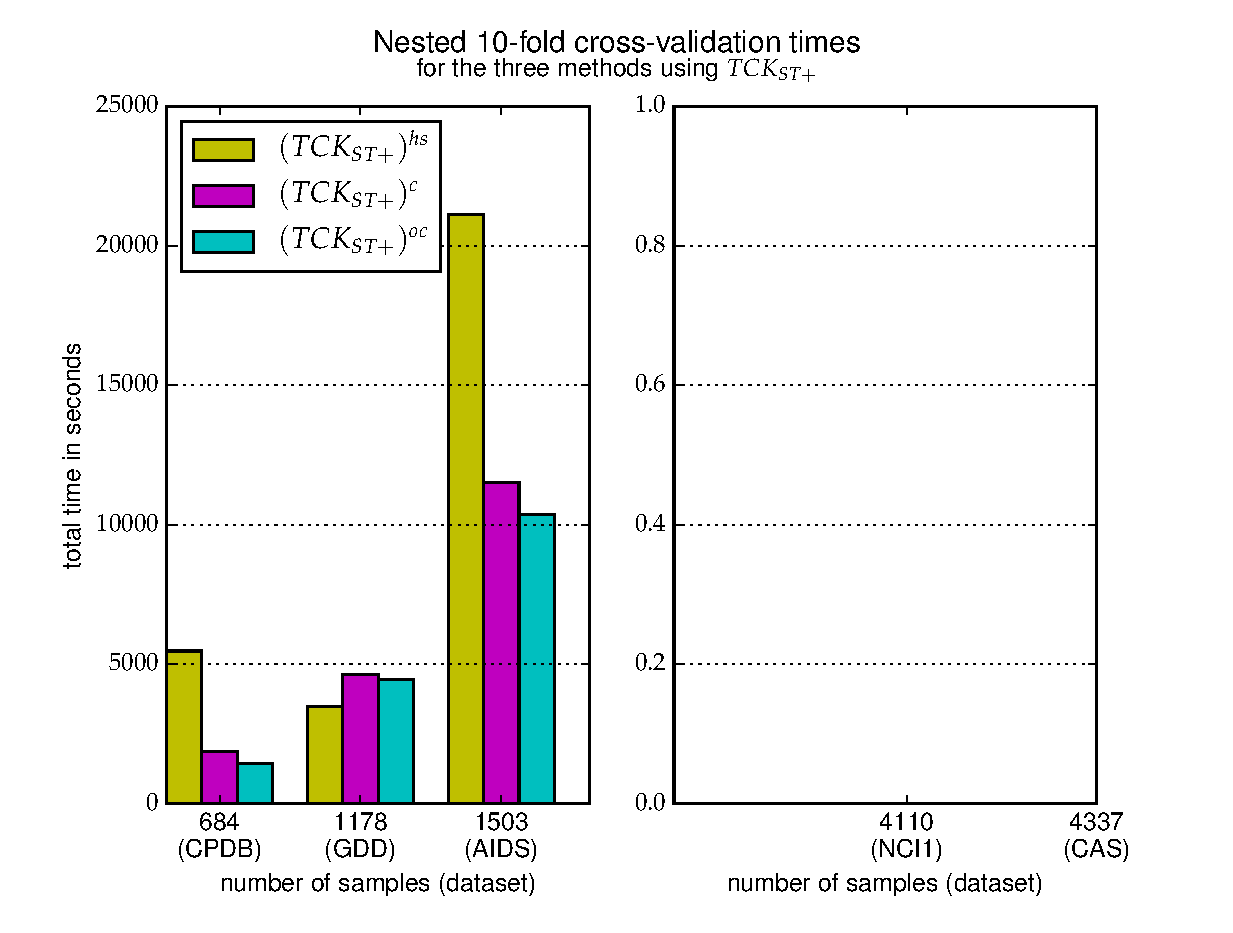
\includegraphics[scale=0.7]{Figures/total_times2}
    \caption{
        This plot shows the time required by each method to compute a full nested 10-fold cross-validation on the benchmark datasets.
        The data shown here refers only to the experiments conducted employing the $TCK_{ST}$ kernel.
    }
    \label{fig:datasetstimes2}
\end{figure}

\begin{figure}[ht]
    \centering
    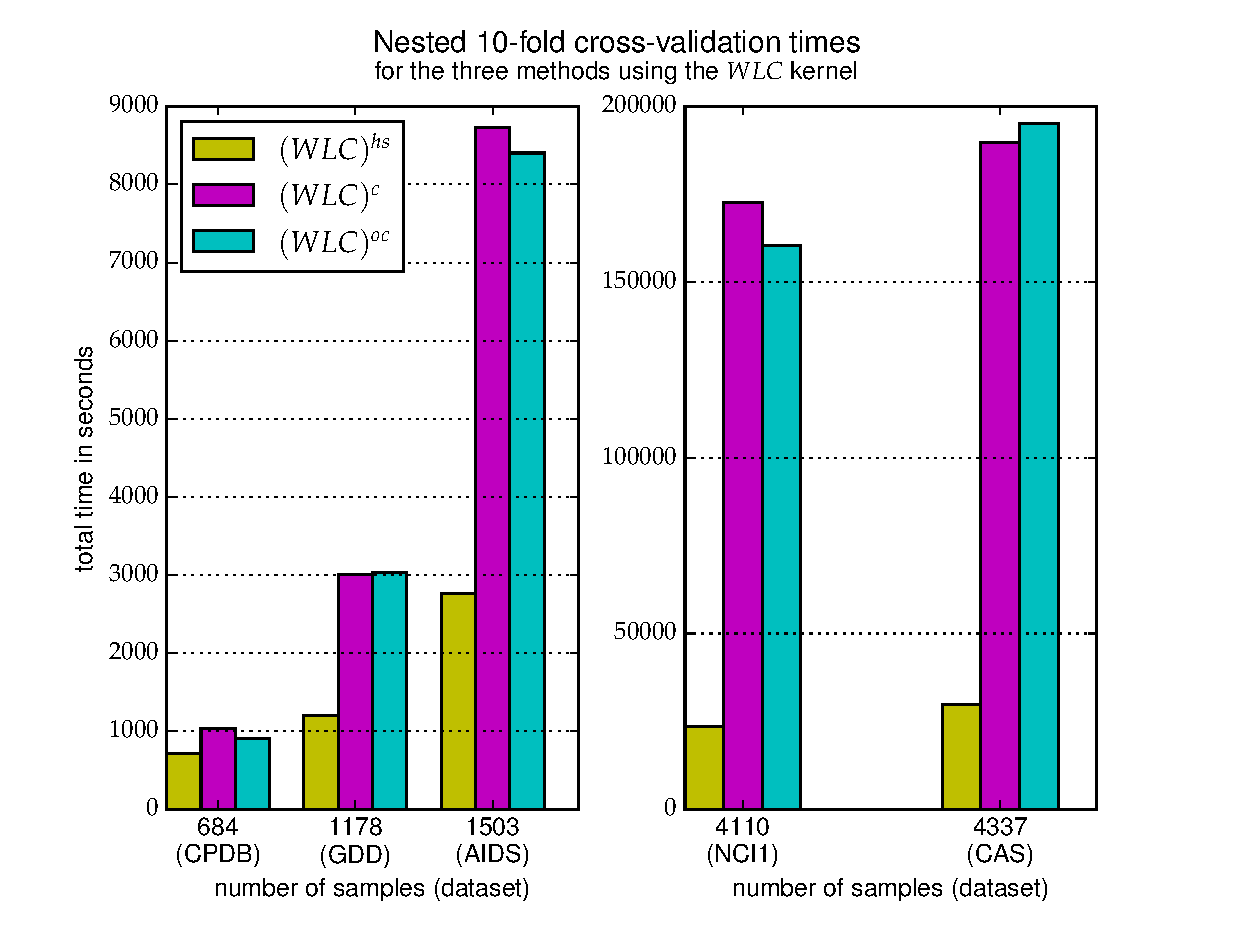
\includegraphics[scale=0.7]{Figures/total_times1}
    \caption{
        This plot shows the time required by each method to compute a full nested 10-fold cross-validation on the benchmark datasets.
        The data shown here refers only to the experiments conducted employing the $WLC$ kernel.
    }
    \label{fig:datasetstimes1}
\end{figure}
%\begin{figure}[ht]
%    \centering
%    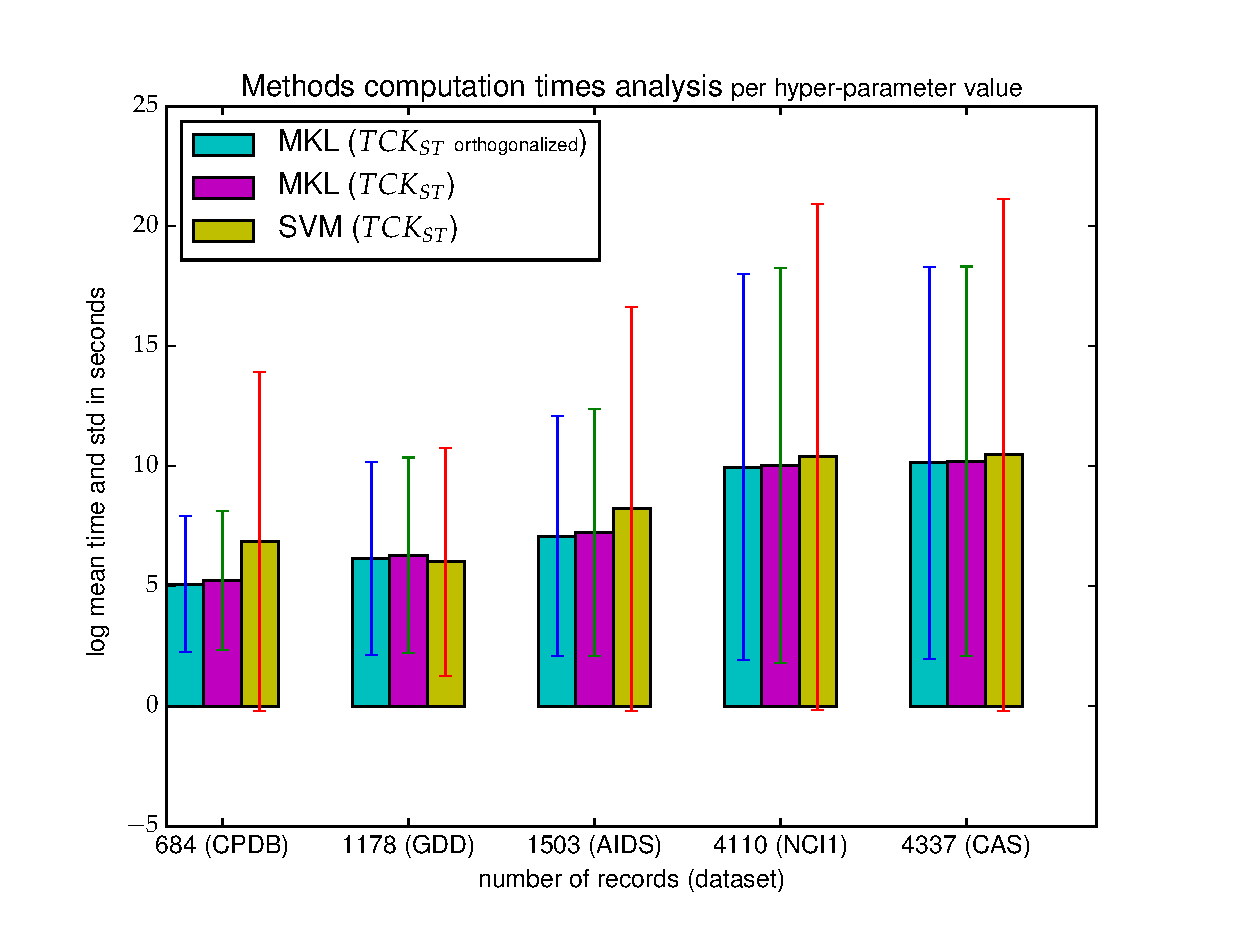
\includegraphics[scale=0.7]{Figures/method_times_avgstd}
%    \caption{
%        This plot shows the mean computation times among all the hyper-parameter values
%        for the classifier, for each learning method and on all the benchmark datasets.
%        Each plot shows the standard deviation among the same set of values plotted as well.
%        The data here represented is taken from the experiments concerning the $TCK_{ST}$ kernel.
%    }
%        \label{fig:meantimes}
%\end{figure}

\subsection{Analysis of model performances}

Here we present the model performance estimates resulting from the experiments described
in Section \ref{sec:description}.
Each table reports the AUROC measure with the standard deviation obtained with
a nested 10-fold cross validation.

Looking at Table \ref{table:results_st}, it is immediately evident how the results
achieved by the proposed methodology are always comparable when not better with respect
to the baseline except when considering the GDD dataset.
$(ODDK_{ST},TCK_{ST})^{oc}$, $(TCK_{ST})^{oc}$, and $(ODDK_{ST})^{oc}$ are the best performers on the NCI1,
AIDS, and CPDB datasets respectively.
On the CAS dataset, the proposed methodology achieves comparable results as the baseline derived from
\cite{gmkl}, i.e $(ODD-MKL)^{hs}$.

As mentioned in Section \ref{subsec:time_results} the GDD dataset represents a rather peculiar case
in which a smaller number of kernels is employed.
EasyMKL is a non-sparse MKL method (Section \ref{subsec:easymkl}) which means that
if the kernels are very similar each one tends to contribute in the same manner to
the final combination, in other words, if combining $R$ identical kernels,
the weights assigned by the algorithm to each kernel would be $\frac{1}{R}$.
On the GDD dataset we are combining a small number of very similar kernels, because
the values considered for the hyper-parameter $h$ are very small.
This, coupled with the rather simple feature space sported by the $ODDK_{ST}$ and 
$TCK_{ST}$ has the effect of a performance deterioration when measured on a 
dataset contained very complex structures as the GDD (Section \ref{subsec:datasets})

Table \ref{table:results_stp} present results in accordance with Table \ref{table:results_st}
beside the case of the GDD dataset in which the $(ODDK_{ST+})^{oc}$ and $(TCK_{ST+})^{oc}$
outperform the baseline.
This data confirms previous results showing that the $ODD_{ST+}$ kernels achieves
comparable or better performances with respect to the $ODD_{ST}$ kernel \cite{dasanmartino2015exploiting}.
The data also confirms the better performances of the $TCK_{ST+}$ on the GDD dataset
with respect to the $TCK_{ST}$ \cite{rtesselli}.

Finally in Table \ref{table:results_wl} we present the results obtained employing the 
kernels derived from the WL framework.
With respect to the previous experiments, in this cases the number of considered
kernels is much lower, i.e. around 10 (see Tables \ref{table:mem1} and \ref{table:mem2}
for a comparison).

From these results it is clear that the WL kernels benefit from being employed with the
proposed method since the performances remain significantly above the baseline
on the AIDS dataset, while remaining very similar on the CAS, CPDB and NCI1 datasets.
A thing worth noting is that these kernel in general seem not to gain any advantage
from being further orthogonalized: in the case of the GDD dataset we even register an
outright performance loss.

From these results we can infer the scarce improvment gained from
using one kernel function and its contextualized version in combination, with or without
the orthogonalization of the feature space.
All the obtained results shows that either both kernels fare at the same level or
one of them dominates the combination outcome.

\begin{landscape}
    \begin{table}[ht]
        \centering
        \begin{tabular}{|l|l|l|l|l|l|}
            \hline
            $\mathrm{(kernels)^{method}}$&CAS&NCI1&AIDS&CPDB&GDD\\
            \hline
            $(ODDK_{ST})^{hs}$&0.8982 $\pm$ 0.0017&0.9069 $\pm$ 0.0010&0.8262 $\pm$ 0.0052&0.8442 $\pm$ 0.0067&0.8473 $\pm$ 0.0038\\
            $(TCK_{ST})^{hs}$&0.9006 $\pm$ 0.0013&0.9150 $\pm$ 0.0011&0.8225 $\pm$ 0.0067&0.8422 $\pm$ 0.0080&\textbf{0.8674 $\pm$ 0.0026}\\
            $(ODDK_{ST} + TCK_{ST})^{hs}$&0.9010 $\pm$ 0.0011&0.9110 $\pm$ 0.0011&0.8323 $\pm$ 0.0065&0.8497 $\pm$ 0.0072&0.8627 $\pm$ 0.0018\\
            $(ODD-MKL_{ST})^{hs}$&\textbf{0.9049 $\pm$ 0.0008}&0.9144 $\pm$ 0.0008&0.8515 $\pm$ 0.0031&0.8564 $\pm$ 0.0056&0.8498 $\pm$ 0.0026\\
            \hline
            $(ODDK_{ST})^c$&0.8899 $\pm$ 0.0013&0.8976 $\pm$ 0.0010 &0.8388 $\pm$ 0.0044&0.8401 $\pm$ 0.0033&0.8013 $\pm$ 0.0019\\
            $(TCK_{ST})^c$&0.8954 $\pm$ 0.0013&0.9095 $\pm$ 0.0006&0.8487 $\pm$ 0.0040&0.8525 $\pm$ 0.0030&0.8617 $\pm$ 0.0022\\
            $(ODDK_{ST}, TCK_{ST})^c$&0.8960 $\pm$  0.0012&0.9076 $\pm$ 0.0007&0.8468 $\pm$ 0.0042&0.8517 $\pm$ 0.0034&0.8612 $\pm$ 0.0018\\
            \hline
            $(ODDK_{ST})^{oc}$&0.9033 $\pm$ 0.0010&0.9195 $\pm$ 0.0006&0.8627 $\pm$ 0.0035&0.8632 $\pm$  0.0029&0.8543 $\pm$ 0.0024\\
            $(TCK_{ST})^{oc}$&0.9036 $\pm$ 0.0010&0.9189 $\pm$ 0.0006&\textbf{0.8634 $\pm$ 0.0034}&0.8625 $\pm$ 0.0032&0.8458 $\pm$ 0.0021\\
            $(ODDK_{ST}, TCK_{ST})^{oc}$&0.9038 $\pm$ 0.0010&\textbf{0.9196 $\pm$ 0.0006}&0.8632 $\pm$ 0.0034&\textbf{0.8632 $\pm$ 0.0038}&0.8528 $\pm$ 0.0022\\
            \hline
        \end{tabular}
        \caption{AUROC results ($\pm$ standard deviation) relative to the experiments
            with the kernels $ODD_{ST}$ and $TCK_{ST}$. Results are
            obtained from a nested 10-fold cross validation.
            Grouping notation is described in Section \ref{subsec:notation}.
            The results of experiments $(ODDK_{ST})^{hs}$ and $(ODD-MKL_{ST})^{hs}$ are taken from \cite{gmkl}.
        }
        \label{table:results_st}
        \medskip

        \begin{tabular}{|l|l|l|l|l|l|}
            \hline
            $\mathrm{(kernels)^{method}}$&CAS&NCI1&AIDS&CPDB&GDD\\
            \hline
            $(ODDK_{ST+})^{hs}$&-&-&-&-&-\\
            $(TCK_{ST+})^{hs}$&0.9008 $\pm$ 0.0017&0.9165 $\pm$ 0.0013&0.8222 $\pm$ 0.0067&0.8462 $\pm$ 0.0048&0.8588 $\pm$ 0.0028\\
            $(ODDK_{ST+} + TCK_{ST+})^{hs}$&0.9022 $\pm$ 0.0015 &0.9163 $\pm$ 0.0011&0.8256 $\pm$ 0.0068&0.8521 $\pm$ 0.0038&0.8570 $\pm$ 0.0043\\
            \hline
            $(ODDK_{ST+})^c$&-&-&0.8489 $\pm$  0.0039&0.8461 $\pm$ 0.0036&0.8178 $\pm$ 0.0022\\
            $(TCK_{ST+})^c$&-&-&0.8503 $\pm$  0.0038&0.8528 $\pm$ 0.0039&0.8645 $\pm$ 0.0018\\
            $(ODDK_{ST+}, TCK_{ST+})^c$&-&-&0.8468 $\pm$ 0.0042&0.8517 $\pm$ 0.0034&0.8612 $\pm$ 0.0018\\
            \hline
            $(ODDK_{ST+})^{oc}$&-&-&0.8628 $\pm$  0.0036&0.8652 $\pm$ 0.0030&\textbf{0.8720 $\pm$ 0.0021}\\
            $(TCK_{ST+})^{oc}$&-&-&\textbf{0.8649 $\pm$  0.0030}&\textbf{0.8666 $\pm$  0.0038}&0.8711 $\pm$ 0.0018 \\
            $(ODDK_{ST+}, TCK_{ST+})^{oc}$&-&-&0.8632 $\pm$  0.0034&0.8632 $\pm$  0.0038&0.8528 $\pm$ 0.0022\\
            \hline
        \end{tabular}
        \caption{AUROC results ($\pm$ standard deviation) of the experiments conducted on
                the $ODD_{ST+}$ kernel and the $TCK_{ST+}$. Results are
                obtained from a nested 10-fold cross validation.
                The notation is analogue to the one of Table \ref{table:results_st} and described in Section \ref{subsec:notation}.}
        \label{table:results_stp}
    \end{table}

    \begin{table}[ht]
        \label{table:results_wl}

        \begin{tabular}{|l|l|l|l|l|l|}
            \hline
            $\mathrm{(kernels)^{method}}$&CAS&NCI1&AIDS&CPDB&GDD\\
            \hline
            $(WL)^{hs}$&0.9015 $\pm$ 0.0020&0.9153 $\pm$ 0.0007&0.8278 $\pm$ 0.0045&0.8548 $\pm$ 0.0063&0.8597 $\pm$ 0.0023\\
            $(WLC)^{hs}$&0.8945 $\pm$ 0.0028&0.9155 $\pm$ 0.0008&0.8274 $\pm$ 0.0056&0.8591 $\pm$ 0.0047&0.7244 $\pm$  0.0039\\
            $(WL + WLC)^{hs}$&0.8995 $\pm$ 0.0020&0.9160 $\pm$ 0.0008&0.8295 $\pm$ 0.0063&0.8518 $\pm$ 0.0056&\textbf{0.8685 $\pm$ 0.0019}\\
            \hline
            $(WL)^c$&0.8984 $\pm$ 0.0016&0.9141 $\pm$ 0.0007&0.8583 $\pm$ 0.0032&0.8566 $\pm$  0.0036&0.8551 $\pm$ 0.0019\\
            $(WLC)^c$&0.9002 $\pm$ 0.0015&0.9174 $\pm$ 0.0008&0.8596 $\pm$ 0.0032&0.8589 $\pm$ 0.0033&0.7263 $\pm$ 0.0036\\
            $(WL, WLC)^c$&\textbf{0.9010 $\pm$ 0.0015}&\textbf{0.9176 $\pm$ 0.0007}&0.8594 $\pm$ 0.0031 &\textbf{0.8597 $\pm$ 0.0032}&0.8583 $\pm$ 0.0015\\
            \hline
            $(WL)^{oc}$&-&-&0.8599 $\pm$ 0.0043&0.8510 $\pm$ 0.0051&0.8175 $\pm$ 0.0015\\
            $(WLC)^{oc}$&-&-&\textbf{0.8603 $\pm$ 0.0044}&0.8499 $\pm$ 0.0046&0.7266 $\pm$ 0.0035\\
            $(WL, WLC)^{oc}$&-&-&0.8602 $\pm$ 0.0043&0.8508 $\pm$ 0.0052&0.8159 $\pm$ 0.0016\\
            \hline
        \end{tabular}
        \caption{AUROC results ($\pm$ standard deviation) relative to the experiments
                conducted with the kernels $WL$ and $WLC$. Results are
                obtained from a nested 10-fold cross validation.
                The notation is analogue to the one of Table \ref{table:results_st} and described in Section \ref{subsec:notation}.}
        \label{table:results_wl}
    \end{table}

\end{landscape}

\section{Kernels Contribution Analysis}
\label{sec:kca}

%EasyMKL finds the optimal linear combination of the kernels it receives in input
%that is, the one that maximizes the separation between the two sets of samples.
%The linear combination is defined as a weighed sum of the kernels;

One point that emerges from the experiments presented here is that the proposed
methodology in general will better perform better when presented with a large number of kernels.
In general a kernel weight reflects its contribution with respect to the
other kernels being combined and it should not be treated as an absolute index
of the goodness of the kernel.

\begin{figure}[ht]
    \centering
    \begin{subfigure}{.45\textwidth}
        \centering
        \includegraphics[width=\linewidth]{Figures/kca_GDD_WL_oc}
        \label{fig:gdd_wloc}
        \caption{}
    \end{subfigure}
    \begin{subfigure}{.45\textwidth}
        \centering
        \includegraphics[width=\linewidth]{Figures/kca_GDD_WLC_oc}
        \label{fig:gdd_wlcoc}
        \caption{}
    \end{subfigure}
    \caption{}
    \label{fig:kca_gdd_wl}
\end{figure}

\begin{figure}[ht]
    \centering
    \begin{subfigure}{.45\textwidth}
        \centering
        \includegraphics[width=\linewidth]{Figures/kca_GDD_ODDST_oc}
        \label{fig:gdd_wloc}
        \caption{}
    \end{subfigure}
    \begin{subfigure}{.45\textwidth}
        \centering
        \includegraphics[width=\linewidth]{Figures/kca_GDD_ODDSTC_oc}
        \label{fig:gdd_wlcoc}
        \caption{}
    \end{subfigure}
    \caption{}
    \label{fig:kca_gdd_wl}
\end{figure}
\begin{figure}[ht]
    \centering
    \begin{subfigure}{.45\textwidth}
        \centering
        \includegraphics[width=\linewidth]{Figures/kca_GDD_ODDSTP_oc}
        \label{fig:gdd_wloc}
        \caption{}
    \end{subfigure}
    \begin{subfigure}{.45\textwidth}
        \centering
        \includegraphics[width=\linewidth]{Figures/kca_GDD_ODDSTP_oc}
        \label{fig:gdd_wlcoc}
        \caption{}
    \end{subfigure}
    \caption{}
    \label{fig:kca_gdd_wl}
\end{figure}

\begin{figure}[ht]
    \centering
    \begin{subfigure}{.45\textwidth}
        \centering
        \includegraphics[width=\linewidth]{Figures/kca_CAS_ODDST_oc}
        \label{fig:gdd_wloc}
        \caption{}
    \end{subfigure}
    \begin{subfigure}{.45\textwidth}
        \centering
        \includegraphics[width=\linewidth]{Figures/kca_CAS_ODDSTC_oc}
        \label{fig:gdd_wlcoc}
        \caption{}
    \end{subfigure}
    \caption{}
    \label{fig:kca_gdd_wl}
\end{figure}

